Este capítulo tem como objetivo apresentar uma discussão acerca dos resultados dos experimentos. Serão expostos o ambiente de experimento, discutido como os modelos reagem à variação dos principais parâmetros, quantidade de divisões, passado visível e tamanho do intervalo do fluxo. Posteriormente, serão apresentados os resultados de como os modelos reagem para a escolha dos hiper-parâmetros selecionados. Além disso, é analisado os resultados das previsões de fluxo de cada modelo nos curtos prazos de 15, 30, 45 e 60 minutos.


\section{Ambiente de Experimento}

O ambiente de experimento foi um servidor equipado com Debian 9, 64 bits. O servidor possui dois CPUs \textit{Intel(R) Xeon(R) Platinum 8160 CPU @ 2.10GHz} e 251 GiB de memória principal. Cada CPU dessas possui 24 núcleos e executa até 48 \textit{threads} em paralelo. Somados são 96 \textit{threads}, que foram usados paralelamente para acelerar a execução do experimento. Porém, em algumas partes da execução, menos \textit{threads} tiveram que ser usadas, pois não havia memória principal o suficiente para todas as instâncias em paralelo.

\section{Resultados das Escolhas de Parâmetros}
\label{section:resultados_parametros}

Após o tratamento dos dados, foram realizados diversos testes para definir os melhores parâmetros de cada modelo. Devido a limitações de hardware os parâmetros foram considerados independentes. Portanto, cada um deles possui um valor padrão e será analisado como esse parâmetro se comporta dado a fixação dos outros. Além disso, essa escolha está sendo feita no pior caso da predição, isto é, na predição de 1h no futuro. Na lista abaixo podem ser vistos os parâmetro que foram levados em consideração nos estudos de caso deste trabalho.

\begin{enumerate}
	\item \textbf{Número de divisões do conjunto de dados} (\textit{Blocking}): Número de divisões utilizadas no blocking para criar mais subconjuntos de dados. Os valores testados foram: 1,2,4,8. Para cada subconjunto, a porcentagem utilizada para treinamento e teste foi a mesma: 80\% para treinamento e 20\% para testes. O valor padrão utilizado foi de 4 divisões.
	\item \textbf{Passado Visível}: Parâmetro que define qual a janela de tempo no passado que será visível no treinamento do modelo. O valor inicial considerado foi de 480 minutos. Os valores de 60, 120, 240 e 480 minutos também foram testados.
	\item \textbf{Tamanho do intervalo do fluxo}: Parâmetro que define o intervalo de tempo no qual será acumulado a quantidade de veículos para o cálculo do fluxo. O valor inicial de teste foi 2,5 minutos. Foram realizados testes para as variações de 5 e 7,5 minutos também (ou 150, 300 e 450 segundos).
\end{enumerate}

\subsection{Número de Divisões do Conjunto de Dados}

Na Figura \ref{figure:res_split}, onde o eixo das ordenadas representa o valor da métrica \acrshort{RMSE} e o eixo das abscissas representa os valores que foram testados para o variável de número de divisões do conjunto,  pode ser observado que todos os modelos apresentaram uma performance melhor que as bases de comparação. Os resultados também são um indicativo que não é necessário um tamanho muito grande de treino para que os modelos se ajustem a distribuição do conjunto de dados. No caso, o melhor número de divisão do conjunto de dados para a maioria os modelos foi  8, como pode ser observado na Tabela \ref{table:res_split}. 

Como o tamanho do conjunto de dados é de 52.992 (intervalo de fluxo padrão foi de 150 segundos), os modelos foram capazes de se ajustar com apenas 5300 dados (aproximadamente), o que seria equivalente a um pouco mais de 1 semana. Os únicos modelos que não apresentaram os melhores médias com o número de divisões igual a 8 foram \textit{\acrshort{SVM}} e \textit{\acrshort{GRU}} que utilizaram a versão A do conjunto de dados. 

Porém, mesmo estes modelos tiveram diferenças pouco significativas se comparados com os seus resultado de 8 divisões. Vale notar também que a maioria dos modelos apresentou uma piora nas predições quando fora utilizado 4 como número de divisão, o que seria equivalente a mais que duas semanas.

\begin{figure}[htbp]
    \centering
    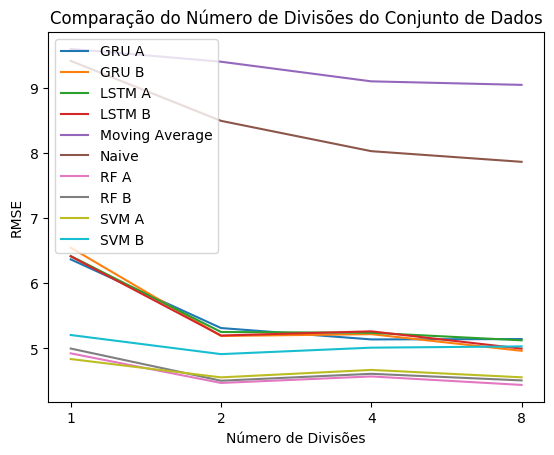
\includegraphics[scale=0.9]{monography/img/comparisons/comparacao_do_numero_de_divisoes_do_conjunto_de_dados_rmse.png}
    \label{figure:res_split}
    \caption[Resposta dos modelos à variação do número de divisões do conjunto de dados]{Resposta dos modelos à variação do número de divisões do conjunto de dados}
\end{figure} 

\begin{table}[htbp]
    \begin{tabular*}{\linewidth}{@{\extracolsep{\fill}}lllll}
    \toprule
     & 
    \multicolumn{1}{l}{\textbf{1}} & 
    \multicolumn{1}{l}{\textbf{2}} &
    \multicolumn{1}{l}{\textbf{4}} &
    \multicolumn{1}{l}{\textbf{8}} \\
    \midrule
    \textbf{MM} & 9.596 $\pm$ 0.000 & 9.399 $\pm$ 0.008 & 9.098 $\pm$ 0.740 & \textbf{9.044} $\pm$ 0.881
    \\
    \midrule
    \textbf{Naive} & 9.413 $\pm$ 0.000 & 8.492 $\pm$ 0.777 & 8.026 $\pm$ 0.868 & \textbf{7.863} $\pm$ 0.889
    \\
    \midrule
    \textbf{RF A} & 4.924 $\pm$ 0.000 & 4.469 $\pm$ 0.254 & 4.569 $\pm$ 0.739 & \textbf{4.439} $\pm$ 0.513
    \\
    \midrule
    \textbf{RF B} & 4.997 $\pm$ 0.000 & 4.504 $\pm$ 0.240 & 4.610 $\pm$ 0.745 & \textbf{4.508} $\pm$ 0.501
    \\
    \midrule
    \textbf{SVM A} & 4.836 $\pm$ 0.000 & \textbf{4.555} $\pm$ 0.160 & 4.669 $\pm$ 0.736 & 4.556 $\pm$ 0.494
    \\
    \midrule
    \textbf{SVM B} & 5.205 $\pm$ 0.000 & \textbf{4.912} $\pm$ 0.042 & 5.011 $\pm$ 0.618 & 5.030 $\pm$ 0.513
    \\
    \midrule
    \textbf{LSTM A} & 6.418 $\pm$ 0.000 & 5.251 $\pm$ 0.279 & 5.239 $\pm$ 0.794 & \textbf{5.123} $\pm$ 0.672
    \\
    \midrule
    \textbf{LSTM B} & 6.412 $\pm$ 0.000 & 5.197 $\pm$ 0.156 & 5.261 $\pm$ 0.830 & \textbf{4.996} $\pm$ 0.696
    \\
    \midrule
    \textbf{GRU A} & 6.366 $\pm$ 0.000 & 5.312 $\pm$ 0.014 & \textbf{5.137} $\pm$ 0.702 & 5.143 $\pm$ 0.516
    \\
    \midrule
    \textbf{GRU B} & 6.545 $\pm$ 0.000 & 5.190 $\pm$ 0.030 & 5.218 $\pm$ 0.686 & \textbf{4.963} $\pm$ 0.643
    \\
    \bottomrule
    \end{tabular*}
    \label{table:res_split}
    \caption{Resultados da Comparação entre os números de divisões. Melhores médias de cada modelo em negrito.}
\end{table}

\subsection{Passado Visível}

\begin{figure}[htbp]
    \centering
    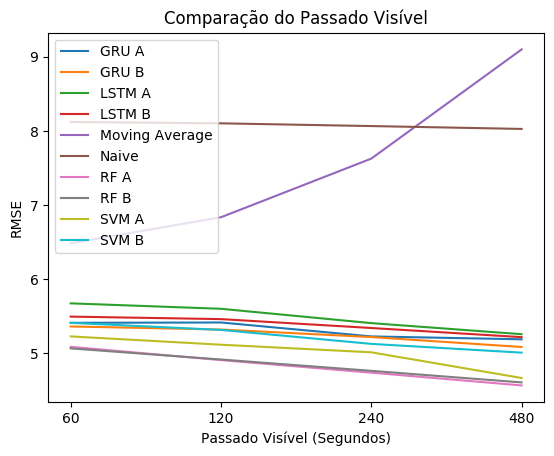
\includegraphics[scale=0.9]{monography/img/comparisons/comparacao_do_passado_visivel_rmse.png}
    \label{figure:res_past}
    \caption[Resposta dos modelos à variação dos valores de passado visível]{Resposta dos modelos à variação dos valores de passado visível}
\end{figure}

\begin{table}[htbp]
    \begin{tabular*}{\linewidth}{@{\extracolsep{\fill}}lllll}
    \toprule
     & 
    \multicolumn{1}{l}{\textbf{60}} & 
    \multicolumn{1}{l}{\textbf{120}} &
    \multicolumn{1}{l}{\textbf{240}} &
    \multicolumn{1}{l}{\textbf{480}} \\
    \midrule
    \textbf{MM} & \textbf{6.485} $\pm$ 0.627 & 6.836 $\pm$ 0.649 & 7.626 $\pm$ 0.684 & 9.098 $\pm$ 0.740
    \\
    \midrule
    \textbf{Naive} & 8.120 $\pm$ 0.869 & \textbf{8.102} $\pm$ 0.873 & 8.065 $\pm$ 0.887 & 8.026 $\pm$ 0.868 
    \\
    \midrule
    \textbf{RF A} & 5.089 $\pm$ 0.758 & 4.910 $\pm$ 0.735 & 4.741 $\pm$ 0.707 & \textbf{4.569} $\pm$ 0.739 
    \\
    \midrule
    \textbf{RF B} & 5.069 $\pm$ 0.753 & 4.918 $\pm$ 0.728 & 4.766 $\pm$ 0.705 & \textbf{4.610} $\pm$ 0.745 
    \\
    \midrule
    \textbf{SVM A} & 5.230 $\pm$ 0.700 & 5.118 $\pm$ 0.706 & 5.015 $\pm$ 0.691 & \textbf{4.669} $\pm$ 0.736 
    \\
    \midrule
    \textbf{SVM B} & 5.412 $\pm$ 0.627 & 5.318 $\pm$ 0.624 & 5.129 $\pm$ 0.586 & \textbf{5.011} $\pm$ 0.618 
    \\
    \midrule
    \textbf{LSTM A} & 5.675 $\pm$ 0.814 & 5.602 $\pm$ 0.713 & 5.409 $\pm$ 0.750 & \textbf{5.260} $\pm$ 0.769 
    \\
    \midrule
    \textbf{LSTM B} & 5.497 $\pm$ 0.563 & 5.463 $\pm$ 0.573 & 5.343 $\pm$ 0.731 & \textbf{5.220} $\pm$ 0.763 
    \\
    \midrule
    \textbf{GRU A} & 5.413 $\pm$ 0.702 & 5.417 $\pm$ 0.650 & 5.230 $\pm$ 0.610 & \textbf{5.191} $\pm$ 0.742 
    \\
    \midrule
    \textbf{GRU B} & 5.364 $\pm$ 0.631 & 5.322 $\pm$ 0.710 & 5.221 $\pm$ 0.747 & \textbf{5.087} $\pm$ 0.679
    \\
    \bottomrule
    \end{tabular*}
    \label{table:res_past}
    \caption{Resultados da Comparação entre as quantidade de passados visíveis. Melhores médias de cada modelo em negrito.}
\end{table}
 

A respeito da variação no quanto do passado o modelo tem acesso, é perceptível na Figura \ref{figure:res_past}, onde o eixo das ordenadas representa o valor da métrica \acrshort{RMSE} e o eixo das abscissas representa os valores que foram testados para o variável de passado visível, que quanto mais acesso ao passado o modelo tiver, melhor será sua predição. Percebe-se também que o melhor valor para a quantidade de acesso do passado, dentre os testados, são 480 minutos (ou 8 horas). 

Porém, é importante ressaltar que mais acesso ao passado também implica em uma quantidade de treino maior, isto é, maior custo computacional, especialmente para modelos de aprendizado profundo, conforme  Figura \ref{figure:passado_visivel_time}, onde o eixo das ordenadas representa o o tempo de treinamento em segundos e o eixo das abscissas representa os valores que foram testados para o variável de passado visível. Dito isso, e considerando que a escala do eixo X é exponencial (Passado visível: 60, 120, 240, 480), pode-se que concluir que para conseguir resultados ainda melhores, seria necessário aumentar de maneira significativa a quantidade de passado visível, o que, talvez, não valesse o aumento do custo computacional, já que, para cada aumento exponencial do eixo X, a qualidade da predição melhora apenas de maneira linear. 

A respeito das bases de comparação, também é claro que o modelo \textit{Naive} não é afetado pela quantidade de tempo de passado visível, mas ainda assim há uma leve mudança no conjunto de dados, pois ao se mudar este parâmetro, o último valor recebido pelo modelo \textit{Naive} é alterado, afetando suas predições e gerando as diferenças vistas na Tabela \ref{table:res_past}. Já o modelo \acrshort{MM} é o único que piora com o tempo. 
\subsection{Tamanho do Intervalo do Fluxo}

Por último, pode-se notar na Figura \ref{figure:res_flow} que o tamanho do intervalo do fluxo adotado impacta de maneira significativa a qualidade das predições dos modelos. Esse efeito pode ser justificado pela quantidade de dados resultantes de cada tamanho do intervalo de fluxo, visto que quanto maior o intervalo, menor a quantidade de dados. 

Por exemplo, são 52.992 dados para 2,5 minutos (150 segundos) e 17.664 para 7.5 minutos (450 segundos). O que torna mais extenso o tempo de treinamento. Dos valores testados, 2.5 minutos é o melhor tamanho de intervalo de fluxo para todos os modelo, como pode ser visto na Tabela \ref{table:res_flow}.

\begin{figure}[H]
    \centering
    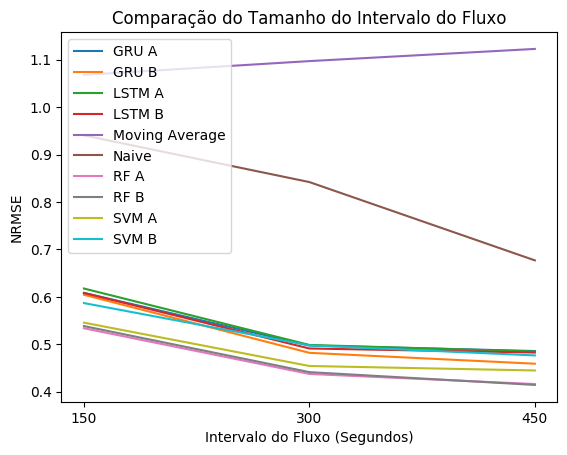
\includegraphics[scale=0.9]{monography/img/comparisons/comparacao_do_tamanho_do_intervalo_do_fluxo_nrmse.png}
    \label{figure:res_flow}
    \caption{Resposta dos modelos à variação dos valores de intervalo de fluxo}
\end{figure}

\begin{table}[H]
    \begin{tabular*}{\linewidth}{@{\extracolsep{\fill}}llll}
    \toprule
     & 
    \multicolumn{1}{l}{\textbf{150}} & 
    \multicolumn{1}{l}{\textbf{300}} &
    \multicolumn{1}{l}{\textbf{450}} \\
    \midrule
    \textbf{MM} & \textbf{9.098} $\pm$ 0.740 & 16.228 $\pm$ 0.875 & 23.233 $\pm$ 1.455
    \\
    \midrule
    \textbf{Naive} & \textbf{8.026} $\pm$ 0.868 & 12.494 $\pm$ 2.059 & 13.954 $\pm$ 1.677
    \\
    \midrule
    \textbf{RF A} & \textbf{4.569} $\pm$ 0.739 & 6.472 $\pm$ 0.464 & 8.582 $\pm$ 1.416
    \\
    \midrule
    \textbf{RF B} & \textbf{4.610} $\pm$ 0.745 & 6.525 $\pm$ 0.383 & 8.543 $\pm$ 1.225
    \\
    \midrule
    \textbf{SVM A} & \textbf{4.669} $\pm$ 0.736 & 6.714 $\pm$ 0.327 & 9.178 $\pm$ 0.955
    \\
    \midrule
    \textbf{SVM B} & \textbf{5.011} $\pm$ 0.618 & 7.361 $\pm$ 0.381 & 9.843 $\pm$ 0.360
    \\
    \midrule
    \textbf{LSTM A} & \textbf{5.269} $\pm$ 0.803 & 7.356 $\pm$ 0.601 & 9.976 $\pm$ 0.802
    \\
    \midrule
    \textbf{LSTM B} & \textbf{5.188} $\pm$ 0.715 & 7.246 $\pm$ 0.631 & 9.929 $\pm$ 0.980
    \\
    \midrule
    \textbf{GRU A} & \textbf{5.183} $\pm$ 0.679 & 7.336 $\pm$ 0.602 & 9.993 $\pm$ 1.034
    \\
    \midrule
    \textbf{GRU B} & \textbf{5.164} $\pm$ 0.758 & 7.106 $\pm$ 0.663 & 9.444 $\pm$ 1.521
    \\
    \bottomrule
    \end{tabular*}
    \label{table:res_flow}
    \caption{Resultados da Comparação entre os intervalos de fluxo. Melhores médias de cada modelo em negrito.}
\end{table}

% Para a escolha do intervalo de fluxo será utilizado uma métrica diferente da utilizada nas outras escolhas. Como essa métrica modifica o tamanho do conjunto de dados e seus valores, será utilizado o \textit{\acrshort{NRMSE}}. Pode-se notar na Figura \ref{figure:res_flow} que o tamanho do intervalo do fluxo adotado impacta de maneira significativa a qualidade das predições dos modelos. Esse efeito pode ser justificado pela oscilação do fluxo que tende a aumentar conforme o intervalo de fluxo diminui. Vale notar que as oscilações diminuem, porém a quantidade de dados disponíveis diminui bastante, por exemplo, são 52.992 dados para 2,5 minutos (150 segundos) e 17.664 para 7.5 minutos (450 segundos). O que torna mais extenso o tempo de treinamento. Dos valores testados, 7.5 minutos é o melhor tamanho de intervalo de fluxo para todos os modelo, como pode ser visto na Tabela \ref{table:res_flow}.

% \begin{figure}[H]
%     \centering
%     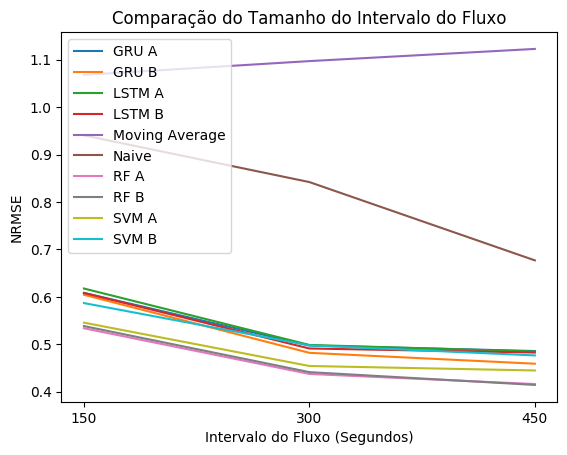
\includegraphics[scale=0.9]{monography/img/comparisons/comparacao_do_tamanho_do_intervalo_do_fluxo_nrmse.png}
%     \label{figure:res_flow}
%     \caption{Resposta dos modelos à variação dos valores de intervalo de fluxo}
% \end{figure}

% \begin{table}[H]
%     \begin{tabular*}{\linewidth}{@{\extracolsep{\fill}}llll}
%     \toprule
%      & 
%     \multicolumn{1}{l}{\textbf{150}} & 
%     \multicolumn{1}{l}{\textbf{300}} &
%     \multicolumn{1}{l}{\textbf{450}} \\
%     \midrule
%     \textbf{MM} & \textbf{1.068} $\pm$ 0.004 & 1.097 $\pm$ 0.021 & 1.122 $\pm$ 0.035
%     \\
%     \midrule
%     \textbf{Naive} & 0.940 $\pm$ 0.036 & 0.842 $\pm$ 0.112 & \textbf{0.677} $\pm$ 0.095
%     \\
%     \midrule
%     \textbf{RF A} & 0.533 $\pm$ 0.048 & 0.437 $\pm$ 0.022 & \textbf{0.416} $\pm$ 0.073
%     \\
%     \midrule
%     \textbf{RF B} & 0.538 $\pm$ 0.047 & 0.441 $\pm$ 0.019 & \textbf{0.414} $\pm$ 0.065
%     \\
%     \midrule
%     \textbf{SVM A} & 0.545 $\pm$ 0.046 & 0.454 $\pm$ 0.017 & \textbf{0.444} $\pm$ 0.052
%     \\
%     \midrule
%     \textbf{SVM B} & 0.586 $\pm$ 0.032 & 0.497 $\pm$ 0.013 & \textbf{0.476} $\pm$ 0.023
%     \\
%     \midrule
%     \textbf{LSTM A} & 0.617 $\pm$ 0.067 & 0.498 $\pm$ 0.048 & \textbf{0.484} $\pm$ 0.060
%     \\
%     \midrule
%     \textbf{LSTM B} & 0.608 $\pm$ 0.056 & 0.491 $\pm$ 0.049 & \textbf{0.482} $\pm$ 0.066
%     \\
%     \midrule
%     \textbf{GRU A} & 0.608 $\pm$ 0.058 & 0.497 $\pm$ 0.049 & \textbf{0.485} $\pm$ 0.069
%     \\
%     \midrule
%     \textbf{GRU B} & 0.604 $\pm$ 0.051 & 0.482 $\pm$ 0.053 & \textbf{0.459} $\pm$ 0.088
%     \\
%     \bottomrule
%     \end{tabular*}
%     \label{table:res_flow}
%     \caption{Resultados da Comparação entre os intervalos de fluxo. Melhores médias de cada modelo em negrito.}
% \end{table}


\section{Comparação dos Resultados Otimizados}

 Por fim, foram realizados testes para otimizar os hiper-parâmetros de cada modelo e garantir as melhores predições. Para alcançar tal objetivo, foi utilizada a técnica de \textit{Grid Search} durante as comparações dos resultados das predições de curto prazo. Abaixo, na figura \ref{figure:pred_no_tuning} podem ser vistos os resultados sem ajuste dos hiper-parâmetros e, na figura \ref{figure:pred_tuning}, com ajuste dos hiper-parâmetros. Os valores exatos dos resultados podem ser vistos nas tabelas  \ref{table:curto_prazo_no_tuning} e \ref{table:curto_prazo_tuning}, para as predições sem e com ajuste, respectivamente. Os valores de parâmetros utilizados para a realização deste teste foram os melhores valores encontrados nos experimentos da seção \ref{section:resultados_parametros}.
 
 Observando a tabela \ref{table:curto_prazo_no_tuning}, é possível constatar que todos os modelos propostos pelo trabalho tiveram performance superior que os modelos utilizados como base de comparação. Dentre esses modelos propostos, o \textit{\acrshort{RF}} foi o que obteve os resultados mais promissores antes do ajuste, se mostrando o melhor modelo em todas as predições de curto prazo, seguido pelo \textit{\acrshort{SVM}}. Os modelos de aprendizado profundo apresentaram os resultados menos satisfatórios, com uma diferença significativa. Porém, este cenário poderia mudar caso o conjunto de dados disponível para o trabalho fosse maior, visto que modelos de aprendizado profundo, como \textit{\acrshort{GRU}} e \textit{\acrshort{LSTM}}, tendem a generalizar melhor à medida que são expostos a um maior volume de dados de treinamento. 

Como dito anteriormente, o modelo que apresentou os melhores médias foi o \textit{\acrshort{RF}}. Entretanto, este cenário muda após o ajuste dos hiper-parâmetros. Como pode ser observado na tabela \ref{table:curto_prazo_tuning}, após a otimização dos resultados, a \textit{\acrshort{SVM}} passou a obter as melhores predições em todos os casos, com uma melhora de cerca de 5\% em relação aos seus resultados antes do ajuste. Os modelos de aprendizado profundo continuaram com resultados menos satisfatórios, porém com uma distância menos significativa. Também é válido notar que todos os outros modelos também obtiveram um aumento de performance, mas não na mesma intensidade. O \textit{\acrshort{RF}}, por exemplo, teve o aumento de performance menos significativo dentre todos os modelos propostos. Isso mostra que os modelos propostos possuem sensibilidades diferentes à variação de hiper-parâmetros.
 
 \begin{figure}[H]
    \centering
    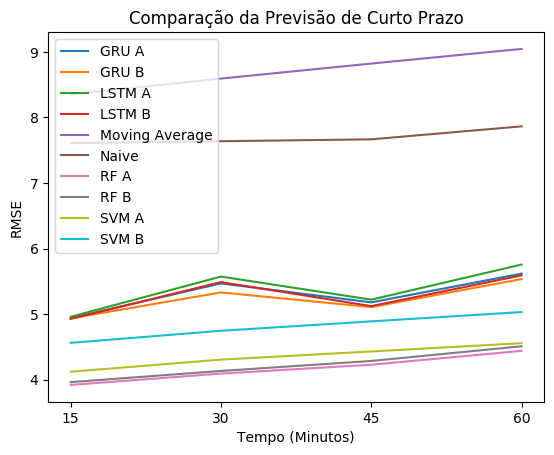
\includegraphics[scale=0.9]{monography/img/comparisons/comparacao_da_previsao_de_curto_prazo_rmse.png}
    \label{figure:pred_no_tuning}
    \caption{Comparação da previsão de curto prazo sem ajuste de hiper-parâmetros}
\end{figure}

\begin{table}[H]
    \begin{tabular*}{\linewidth}{@{\extracolsep{\fill}}lllll}
    \toprule
     & 
    \multicolumn{1}{l}{\textbf{15 mins}} & 
    \multicolumn{1}{l}{\textbf{30 mins}} &
    \multicolumn{1}{l}{\textbf{45 mins}} &
    \multicolumn{1}{l}{\textbf{60 mins}} \\
\midrule
\textbf{MM} & 8.352 $\pm$ 0.820 & 8.592 $\pm$ 0.846 & 8.821 $\pm$ 0.866 & 9.044 $\pm$ 0.881
\\

\midrule
\textbf{Naive} & 7.607 $\pm$ 0.993 & 7.636 $\pm$ 0.839 & 7.665 $\pm$ 0.768 & 7.863 $\pm$ 0.889
\\

\midrule
\textbf{RF A} & \textbf{3.919 $\pm$ 0.395} & \textbf{4.092 $\pm$ 0.409} & \textbf{4.227 $\pm$ 0.467} & \textbf{4.439 $\pm$ 0.513}
\\

\midrule
\textbf{RF B} & 3.962 $\pm$ 0.400 & 4.132 $\pm$ 0.410 & 4.284 $\pm$ 0.468 & 4.508 $\pm$ 0.501
\\

\midrule
\textbf{SVM A} & 4.120 $\pm$ 0.457 & 4.305 $\pm$ 0.466 & 4.429 $\pm$ 0.491 & 4.556 $\pm$ 0.494
\\

\midrule
\textbf{SVM B} & 4.560 $\pm$ 0.465 & 4.745 $\pm$ 0.478 & 4.888 $\pm$ 0.506 & 5.030 $\pm$ 0.513
\\

\midrule
\textbf{LSTM A} & 4.958 $\pm$ 0.579 & 5.571 $\pm$ 0.539 & 5.219 $\pm$ 0.527 & 5.755 $\pm$ 0.448
\\

\midrule
\textbf{LSTM B} & 4.926 $\pm$ 0.567 & 5.487 $\pm$ 0.577 & 5.121 $\pm$ 0.582 & 5.590 $\pm$ 0.596
\\

\midrule
\textbf{GRU A} & 4.937 $\pm$ 0.579 & 5.467 $\pm$ 0.548 & 5.178 $\pm$ 0.585 & 5.616 $\pm$ 0.537
\\

\midrule
\textbf{GRU B} & 4.934 $\pm$ 0.628 & 5.330 $\pm$ 0.473 & 5.106 $\pm$ 0.619 & 5.534 $\pm$ 0.542
\\
    \bottomrule
    \end{tabular*}
    \label{table:curto_prazo_no_tuning}
    \caption{Resultados das predições de curto prazo dos modelos sem ajuste de hiper-parâmetros.}
\end{table}

\begin{figure}[H]
    \centering
    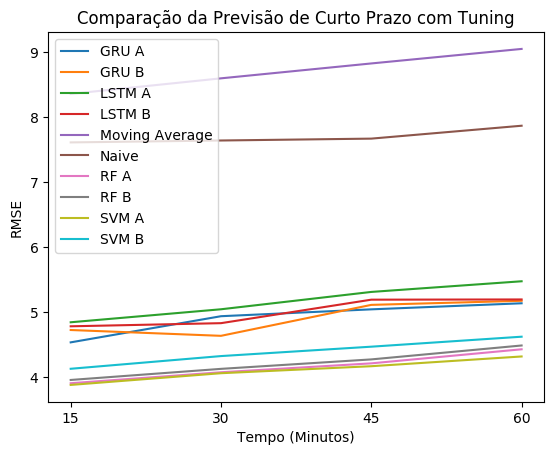
\includegraphics[scale=0.9]{monography/img/comparisons/comparacao_da_previsao_de_curto_prazo_com_tuning_rmse.png}
    \label{figure:pred_tuning}
    \caption{Comparação da previsão de curto prazo com ajuste de hiper-parâmetros}
\end{figure}

\begin{table}[H]
    \begin{tabular*}{\linewidth}{@{\extracolsep{\fill}}lllll}
    \toprule
     & 
    \multicolumn{1}{l}{\textbf{15 mins}} & 
    \multicolumn{1}{l}{\textbf{30 mins}} &
    \multicolumn{1}{l}{\textbf{45 mins}} &
    \multicolumn{1}{l}{\textbf{60 mins}} \\
\midrule
\textbf{MM} & 8.352 $\pm$ 0.820 & 8.592 $\pm$ 0.846 & 8.821 $\pm$ 0.866 & 9.044 $\pm$ 0.881
\\
\midrule
\textbf{Naive} & 7.607 $\pm$ 0.993 & 7.636 $\pm$ 0.839 & 7.665 $\pm$ 0.768 & 7.863 $\pm$ 0.889
\\
\midrule
\textbf{RF A} & 3.904 $\pm$ 0.399 & 4.073 $\pm$ 0.422 & 4.210 $\pm$ 0.466 & 4.426 $\pm$ 0.512
\\
\midrule
\textbf{RF B} & 3.954 $\pm$ 0.397 & 4.125 $\pm$ 0.409 & 4.270 $\pm$ 0.474 & 4.484 $\pm$ 0.503
\\
\midrule
\textbf{SVM A} & \textbf{3.878 $\pm$ 0.423} & \textbf{4.058 $\pm$ 0.443} & \textbf{4.166 $\pm$ 0.486} & \textbf{4.315 $\pm$ 0.530}
\\
\midrule
\textbf{SVM B} & 4.126 $\pm$ 0.336 & 4.321 $\pm$ 0.384 & 4.466 $\pm$ 0.469 & 4.619 $\pm$ 0.523
\\
\midrule
\textbf{LSTM A} & 4.841 $\pm$ 0.625 & 5.041 $\pm$ 0.533 & 5.308 $\pm$ 0.379 & 5.472 $\pm$ 0.505
\\
\midrule
\textbf{LSTM B} & 4.779 $\pm$ 0.562 & 4.827 $\pm$ 0.559 & 5.189 $\pm$ 0.601 & 5.192 $\pm$ 0.691
\\
\midrule
\textbf{GRU A} & 4.532 $\pm$ 0.552 & 4.934 $\pm$ 0.306 & 5.040 $\pm$ 0.536 & 5.133 $\pm$ 0.487
\\
\midrule
\textbf{GRU B} & 4.722 $\pm$ 0.672 & 4.633 $\pm$ 0.420 & 5.109 $\pm$ 0.660 & 5.171 $\pm$ 0.537
\\
    \bottomrule
    \end{tabular*}
    \label{table:curto_prazo_tuning}
    \caption{Resultados das predições de curto prazo dos modelos com ajuste de hiper-parâmetros.}
\end{table}

\subsection{Análise dos hiper-parâmetros escolhidos}

Nos métodos de aprendizado profundo, ao observar a tabela \ref{table:best_hiper_deep}, pode-se notar que para os modelos que utilizam o conjunto de dados A, são necessárias menos células na rede, o que é coerente com a teoria, visto que o conjunto de dados A possui menos atributos e, consequentemente, menos informações para processar.

Observando os resultados da escolha de hiper-parâmetros, como observado na Tabela \ref{table:best_hiper_deep}, é perceptível que os modelos de aprendizado profundo não precisaram de uma taxa de aprendizado tão alta para aprender a distribuição dos dados. Porém, há uma diferença para os resultados quando os modelos utilizam o conjunto de dados A, ou B. O \textit{\acrshort{LSTM}}, por exemplo, possui a mesma taxa de aprendizado para os dois conjuntos de dados, mas a quantidade de células necessárias do conjunto B é maior, o que mostra que mesmo com uma taxa de aprendizado igual, o conjunto de dados com maior número de informações também necessita de mais processamento para generalizar. Este padrão também se mantém com o \textit{\acrshort{GRU}}, onde a taxa de aprendizado para o modelo que utiliza o conjunto de dados B chegou a ser menor que o utilizado pelo modelo A, mas, da mesma forma que acontece com o \textit{\acrshort{LSTM}}, a quantidade de células necessárias na rede foi o dobro que o utilizado pelo modelo A.

\begin{table}[H]
    \begin{tabular*}{\linewidth}{@{\extracolsep{\fill}}lll}
    \toprule
     & 
    \multicolumn{1}{l}{\textbf{Taxa de Aprendizado}} & 
    \multicolumn{1}{l}{\textbf{Células}} 
    \\
\midrule
\textbf{LSTM A} & 0.004 & 50\\ \midrule
\textbf{LSTM B} & 0.004 & 125 \\ \midrule
\textbf{GRU A} & 0.016 &  75 \\ \midrule
\textbf{GRU B} & 0.008 &  125 \\
    \bottomrule
    \end{tabular*}
    \label{table:best_hiper_deep}
    \caption{Valores de hiper-parâmetros mais recorrentes no \textit{Grid Search} para os modelos de aprendizado profundo.}
\end{table}

Como pode ser observado na Tabela \ref{table:best_hiper_svm}, o erro escolhido foi mais alto para o banco de dados B, indicando uma dificuldade maior do modelo de se ajustar quando está usando um conjunto de dados com mais atributos. Nos testes realizados, a escolha do Gamma (\(\gamma\)) foi unânime. Mas vale notar que o \(\gamma\) não é o mesmo para o \textit{\acrshort{SVM}} que usa o banco de dados A e para o que usa o banco de dados B. Isso acontece, pois o valor \textit{scale} da biblioteca calcula o valor do \(\gamma\) baseado na variância do conjunto de testes, mais especificamente \(\frac{1}{n * var_X}\), com \(n\) sendo o número de atributos e \(var_X\) a variância do conjunto de testes.

\begin{table}[H]
    \begin{tabular*}{\linewidth}{@{\extracolsep{\fill}}lll}
    \toprule
     & 
    \multicolumn{1}{l}{\textbf{C}} & 
    \multicolumn{1}{l}{\textbf{Gamma}} 
    \\
\midrule
\textbf{SVM A} & 10 & scale\\ \midrule
\textbf{SVM B} & 100 & scale \\ \midrule

    \bottomrule
    \end{tabular*}
    \label{table:best_hiper_svm}
    \caption{Valores de hiper-parâmetros mais recorrentes no \textit{Grid Search} para o \textit{\acrshort{SVM}}}
\end{table}

Para o \textit{\acrshort{RF}}, como visto anteriormente, não houve uma melhora significativa em suas predições mesmo dobrando o número de árvores e tornando o modelo menos prono a sobre-ajuste ao limitar a altura máxima, como pode ser visto na Tabela \ref{table:best_hiper_rf}. Nota-se também que o tempo necessário para treiná-lo com o conjunto de dados B aumentou consideravelmente ao se realizar o ajuste de hiper-parâmetros, tornando o modelo o mais custoso computacionalmente, conforme pode ser visto na Figura
\ref{figure:previsao_de_curto_prazo_com_tuning_time}.

\begin{table}[H]
    \begin{tabular*}{\linewidth}{@{\extracolsep{\fill}}lll}
    \toprule
     & 
    \multicolumn{1}{l}{\textbf{Altura Máx. Arvore}} & 
    \multicolumn{1}{l}{\textbf{Nr. Estimadores}} 
    \\
\midrule
\textbf{RF A} & 32 & 800\\ \midrule
\textbf{RF B} & 32 & 800 \\ \midrule

    \bottomrule
    \end{tabular*}
    \label{table:best_hiper_rf}
    \caption{Valores de hiper-parâmetros mais recorrentes no \textit{Grid Search} para o \textit{\acrshort{RF}}.}
\end{table}

\section{Precisão}

 %Nesse trabalho, as predições também foram avaliadas como se, em vez de um problema de regressão, houvesse um problema de classificação. Para isto, avaliou-se se os modelos, mesmo errando as predições, seriam capazes de acertar se o fluxo vai aumentar ou diminuir. Entretanto, utilizando essa métrica, os modelos não alcançaram uma performance satisfatória, ficando com acurácia por volta de 60\%. Com \textit{\acrshort{SVM}} e \textit{\acrshort{RF}} atingindo, às vezes, a casa dos 70\% de acurácia. A grande variância dessa métrica dos modelos pode ter sido causada devido ao grande ruído existente nos dados ao se utilizar o agrupamento de fluxo de 150 segundos, onde em um minuto tem-se s 30 veículos passando e, no minuto seguinte, 0 veículos passando. Os resultados sem ajuste de hiper-parâmetros podem ser observados nas Figuras \ref{figure:comparacao_previsao_precisao_15_sem_tuning}, \ref{figure:comparacao_previsao_precisao_30_sem_tuning}, \ref{figure:comparacao_previsao_precisao_45_sem_tuning}e
%\ref{figure:comparacao_previsao_precisao_60_sem_tuning}. Já os os que possuem podem ser observados nas Figuras 
%\ref{figure:comparacao_previsao_precisao_15_com_tuning},
%\ref{figure:comparacao_previsao_precisao_30_com_tuning},
%\ref{figure:comparacao_previsao_precisao_45_com_tuning} e

Nesse trabalho, as predições também foram avaliadas como se, em vez de um problema de regressão, houvesse um problema de classificação. Para isto, avaliou-se se os modelos, mesmo errando as predições, seriam capazes de acertar se o fluxo vai aumentar ou diminuir. Entretanto, utilizando essa métrica, os modelos não alcançaram uma performance satisfatória, ficando com acurácia por volta de 55\%. Com \textit{\acrshort{SVM}} e \textit{\acrshort{RF}} atingindo, às vezes, a casa dos 65\% de acurácia. A grande variância dessa métrica dos modelos pode ter sido causada devido ao grande ruído existente nos dados ao se utilizar o agrupamento de fluxo de 150 segundos, onde em um minuto tem-se s 30 veículos passando e, no minuto seguinte, 0 veículos passando. 

\begin{figure}[H]
    \centering
    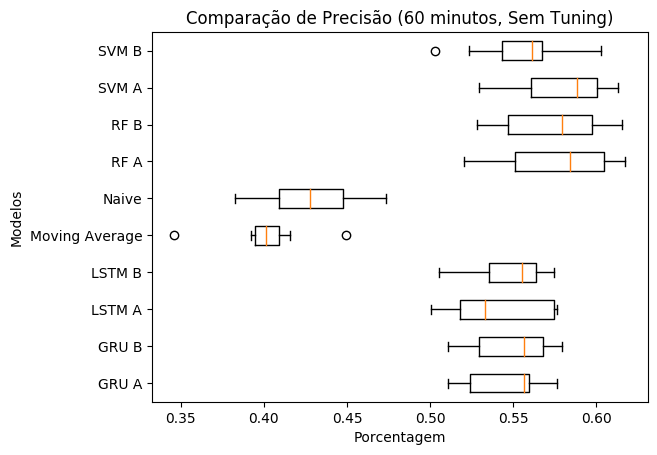
\includegraphics[scale=0.8]{monography/img/snapshots/comparacao_de_precisao_(60_minutos,_sem_tuning)_performance_boxes.png}
    \label{figure:comparacao_previsao_precisao_60_sem_tuning_r}
    \caption{Comparação de precisão em previsão de fluxo de 60 minutos sem ajuste de hiper-parâmetros}
\end{figure}

Nota-se que os modelos que apresentaram as melhores predições nos testes anteriores também são os modelos que possuem a maior capacidade de predizer se o fluxo de veículos tende a aumentar, ou diminuir. Para os resultados antes do \textit{Tuning}, observa-se na figura \ref{figure:comparacao_previsao_precisao_60_sem_tuning_r} que o \acrshort{SVM} apresenta os melhores resultados, seguido do \acrshort{RF}.

\begin{figure}[H]
    \centering
    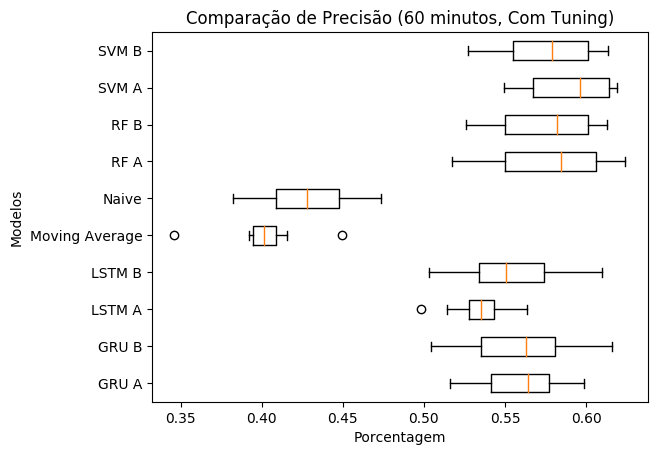
\includegraphics[scale=0.8]{monography/img/snapshots/comparacao_de_precisao_(60_minutos,_com_tuning)_performance_boxes.png}
    \label{figure:comparacao_previsao_precisao_60_com_tuning_r}
    \caption{Comparação de precisão em previsão de fluxo de 60 minutos com ajuste de hiper-parâmetros}
\end{figure}

Após o \textit{Tuning}, é perceptível na figura \ref{figure:comparacao_previsao_precisao_60_com_tuning_r} a melhora de performance de todos os modelos, em especial o \acrshort{SVM}, que continuou a obter os melhores resultados. Também é importante observar que todos os modelos propostos obtiveram um melhor desempenho que as bases de comparação por uma margem significativa.

\section{Observações}

Quanto ao \textit{\acrshort{MAE}}, os resultados apresentados foram muito similares aos do \textit{\acrshort{RMSE}}, como pode ser observado nas figuras \ref{figure:previsao_de_curto_prazo_mae_r} e \ref{figure:previsao_de_curto_prazo_com_tuning_mae_r} abaixo.

\begin{figure}[H]
    \centering
    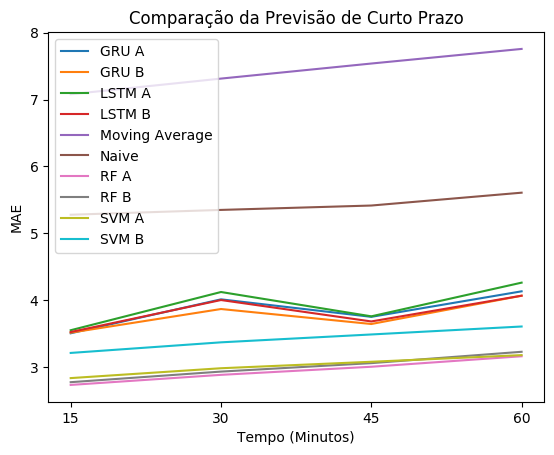
\includegraphics[scale=0.8]{monography/img/comparisons/comparacao_da_previsao_de_curto_prazo_mae.png}
    \label{figure:previsao_de_curto_prazo_mae_r}
    \caption{Comparação de previsão de curto prazo sem ajuste de hiper-parâmetros utilizando MAE}
\end{figure}

\begin{figure}[H]
    \centering
    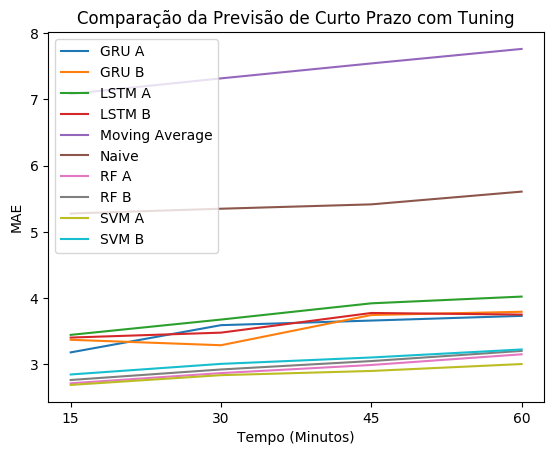
\includegraphics[scale=0.8]{monography/img/comparisons/comparacao_da_previsao_de_curto_prazo_com_tuning_mae.png}
    \label{figure:previsao_de_curto_prazo_com_tuning_mae_r}
    \caption{Comparação de previsão de curto prazo com ajuste de hiper-parâmetros utilizando MAE}
\end{figure}